\documentclass[11pt]{article}
\usepackage[margin=1in]{geometry}
\usepackage[T1]{fontenc}
\usepackage{lmodern}
\usepackage{amsmath,amssymb}
\usepackage{booktabs}
\usepackage{graphicx}
\usepackage[hidelinks]{hyperref}
\usepackage{xcolor}
\usepackage{enumitem}
\setlist{nosep,leftmargin=1.4em}
\newcommand{\ledger}[1]{\href{https://github.com/Royer-Research-Labs/Dilution-Attention/blob/main/docs/signals.md}{#1}}
\graphicspath{{../figures/}}

\title{DilutionAttention: a parameter-free attention operator that divides each bid by the demand its key has already absorbed\\[4pt]\large Technical report, version 0.1}
\author{Nick Royer\\Royer Research Labs, LLC\\\small\url{https://github.com/Royer-Research-Labs/Dilution-Attention}\\\small software: \href{https://doi.org/10.5281/zenodo.23073037}{doi:10.5281/zenodo.23073037}}
\date{September 2026}

\begin{document}
\maketitle

\begin{abstract}
We describe \emph{dilution attention}, a causal attention operator with no learnable parameters.
Each query's softmax bid on a key is divided by the cumulative demand that key has already received
from earlier queries, and the resulting shares are renormalised. The operator is an exact
reformulation of inclusive temporal attention applied to row-normalised scores, used here as the
attention of a causal Transformer language model. At 209M parameters, trained at a 16K-token context
on a Chinchilla-matched budget with \emph{no position encoding}, dilution models retrieve planted
keywords at eight times their training context in both seeds, where softmax models trained
identically reach 0.17--0.19 at their own context and chance beyond it. On long books, dilution's
loss stays flat to eight times its training context while every softmax model's rises steeply, and
past the trained context every softmax model we tested writes incoherent text while dilution's
samples keep their in-context quality. Inside the trained context, dilution's loss and judged sample
quality track the stronger softmax-with-RoPE control on in-domain text (level at 16K, behind it at
1K), but on out-of-domain books it trails that control by 0.05--0.24 nats. We release fused Triton kernels with exact
gradients, the training and evaluation code, run records for the 101 training runs behind the
published results, the weights of 16 models and an evidence ledger, and we state the limits: a 209M scale, a synthetic
retrieval test, and training about 2.2$\times$ slower than softmax at 16K.
\end{abstract}

\section{Introduction}

Softmax attention distributes a fixed budget of weight over the visible keys, and nothing records how
much of that budget other queries have already spent on a key. Trained models use this freedom in
recognisable ways: they park unneeded mass on a few positions, usually the first token (the
\emph{attention sink}~\cite{streamingllm,stablemask}), and they depend on position encodings whose
behaviour outside the trained range limits length generalisation~\cite{rope,nope,pi,yarn}.

Dilution attention adds a price. A query still places softmax bids, but each bid is divided by the
demand its key has accumulated from earlier queries, so a key that many queries have already claimed
yields a smaller share. The idea has a close precedent: temporal attention in recurrent
encoder--decoders divides the current alignment by the alignments of earlier decoder steps
\cite{sankaran,paulus}. Our contribution is not that division; it is (i)~an inclusive, row-calibrated
form that is well defined in causal self-attention, where the exclusive form degenerates; (ii)~fused
kernels with exact gradients that train it at 16K-token contexts and run it forward to 256K tokens; and (iii)~a controlled
empirical study, with matched softmax baselines and position-encoding controls, of what it does to
loss, retrieval, generation and attention structure.

The central empirical result is length extrapolation without position encoding
(Figure~\ref{fig:retrieval}). The comparison that isolates the operator holds everything else fixed:
the same architecture, data, schedule and learning rate, and no position encoding on either side.
We report every seed, including the ones that make the story less tidy: extrapolation range varies by
seed even when loss replicates to three decimals.

\section{The operator}

For causal logits $z_{ij} = q_i \cdot k_j/\sqrt{d}$, $j \le i$:
\begin{align}
p_{ij} &= \frac{\exp z_{ij}}{\sum_{k \le i} \exp z_{ik}} && \text{softmax bids}\\
d_{ij} &= \sum_{r \le i} p_{rj} && \text{demand on key } j \text{ (inclusive)}\\
s_{ij} &= \frac{p_{ij}}{d_{ij} + \epsilon}, \qquad
A_{ij} = \frac{s_{ij}}{\sum_{k \le i} s_{ik}}, \qquad
o_i = \sum_{j \le i} A_{ij} v_j .
\end{align}
The operator has no parameters, is causal, is invariant to shifting a row's logits, and keeps every
pre-normalisation share in $[0,1]$ (the diagonal share is exactly $p_{ii}/(0 + p_{ii}) = 1$ up to
$\epsilon$). It is $O(T^2)$ like softmax attention. Cached decoding needs the KV cache plus one fp32
demand accumulator per key and head.

\paragraph{Relation to temporal attention.} Writing $z'_{ij} = \log p_{ij}$, the share is
$s_{ij} = \exp z'_{ij} / \sum_{r \le i} \exp z'_{rj}$: dilution is inclusive temporal attention on
row-calibrated logits. Temporal attention~\cite{sankaran,paulus} divides by \emph{exclusive} history,
$\sum_{r<i}$. In causal self-attention that denominator is exactly zero at each key's first query,
which is the key itself, so the diagonal wins every row by $1/\epsilon$ and attention collapses to the
identity at initialisation. A model trained with exclusive history (and row-normalised bids) escapes
the collapse in every layer but the first, which stays an identity map. Against inclusive dilution
trained with the same recipe it loses 0.072 nats, and retrieval at 7.9K tokens falls from 1.00 to
0.62, no better than a control with no demand step at all (64M, one seed each; \ledger{S18}). The
raw-exponential cells of the temporal-attention factorial remain untested: our fp32 implementation
overflowed, and a numerically stable cumulative-logsumexp form has not been built.

\paragraph{Softmax bids work best of those tested.} The share's gradient scales as $1/p$. Of the bid functions
tried, only softmax and sigmoid train; sigmoid is 0.33 nats worse. Bids whose Jacobian lacks a factor
of the bid (ReLU, ReLU$^2$, a min-shifted linear bid) diverge, as that predicts. Softplus also
diverged although its Jacobian does carry the factor; that failure is measured, not explained. With
softmax bids the demand step is worth 0.178 nats and lifts retrieval at 7.9K from 0.59 to 1.00
(64M, learning-rate matched; \ledger{S3, S4}).

\section{Implementation}

The column prefix sum is the operator's only sequential coupling, so standard fused-attention
kernels cannot express it as a score modifier. Our Triton kernels compute online softmax statistics,
then a key-parallel pass that carries demand in registers and saves checkpoints every 32 rows; the
backward walks row blocks in reverse, so the per-key demand suffix is a running sum, and applies the
softmax-Jacobian correction in a separate pass. Gradients are exact; a variant that treated demand as
a constant in the backward was 23\% faster and trained an unstable objective (\ledger{S26}). Forward
plus backward takes 5.46\,ms at batch 8, 8 heads, 4K tokens and 30.2\,ms at the 209M training shape
(2 sequences, 12 heads, 16K tokens) on an RTX PRO 6000; a 256K-token forward runs in 17.9\,GiB.
Softmax attention (SDPA) trains 1.3$\times$ faster than dilution at 1K context and 2.2$\times$ faster at
16K. A full-schedule replay reproduced the loss of the first working kernels to 0.0007 nats.

\section{Experimental setup}

\paragraph{Models.} Decoder-only Transformers with SwiGLU MLPs, no biases, tied embeddings and the
GPT-2 vocabulary: a 64M family (12 layers, width 512, 8 heads) and a 209M family (24 layers, width
768, 12 heads). Arms differ only in the attention operator and position encoding: all-dilution with
no position encoding; all-softmax with RoPE (base $5\times10^5$) or with none; \emph{alt6}, which
alternates RoPE-softmax layers with unrotated dilution layers; and, at 64M, dilution with RoPE on
alternate layers. Dilution adds no parameters, so matched arms have identical parameter counts.

\paragraph{Training.} FineWeb-Edu~\cite{fineweb} (a 40B-token GPT-2-tokenised sample), 65,536 tokens
per step at 209M, learning rate $6\times10^{-4}$, cosine over a 2$\times$-Chinchilla~\cite{chinchilla}
schedule of 8.4B tokens. ``1$\times$'' is the step-64,000 checkpoint (4.19B tokens; learning rate 55.7\%
of peak); ``2$\times$'' is the end of the schedule. The 209M models are trained at 16K and at 1K
context, two seeds per arm; the 64M reliability studies use three seeds.

\paragraph{Evaluation.} \emph{Loss}: one common validation slice per scale, because in-run windows
differ with batch size. \emph{Retrieval (NIAH)}: a synthetic, likelihood-scored test; a fixed
54-token paragraph is repeated to length, the sentence ``The secret keyword is $w$.'' is planted at
evenly spaced depths, and the model's likelihood is compared across 8 fixed single-token keywords,
of which the one the model prefers on a needle-free prompt is disqualified, so chance is 1/7. It
measures copying one planted token out of repetitive filler, not reasoning. Beyond the trained
context, RoPE layers use dynamic NTK base scaling~\cite{yarn}. \emph{Long-document perplexity}: loss
by position on PG-19 books~\cite{pg19} (Section~\ref{sec:pg19}). \emph{Generation}: 256-token
continuations of validation prompts, scored in bits per byte by a larger judge model,
SmolLM2-1.7B~\cite{smollm2}, which sees only the last 4,096 tokens of each prompt; paired over
prompts and read together with repetition~\cite{unlikelihood,nucleus}.

\section{Results}

\begin{figure}[t]
\centering
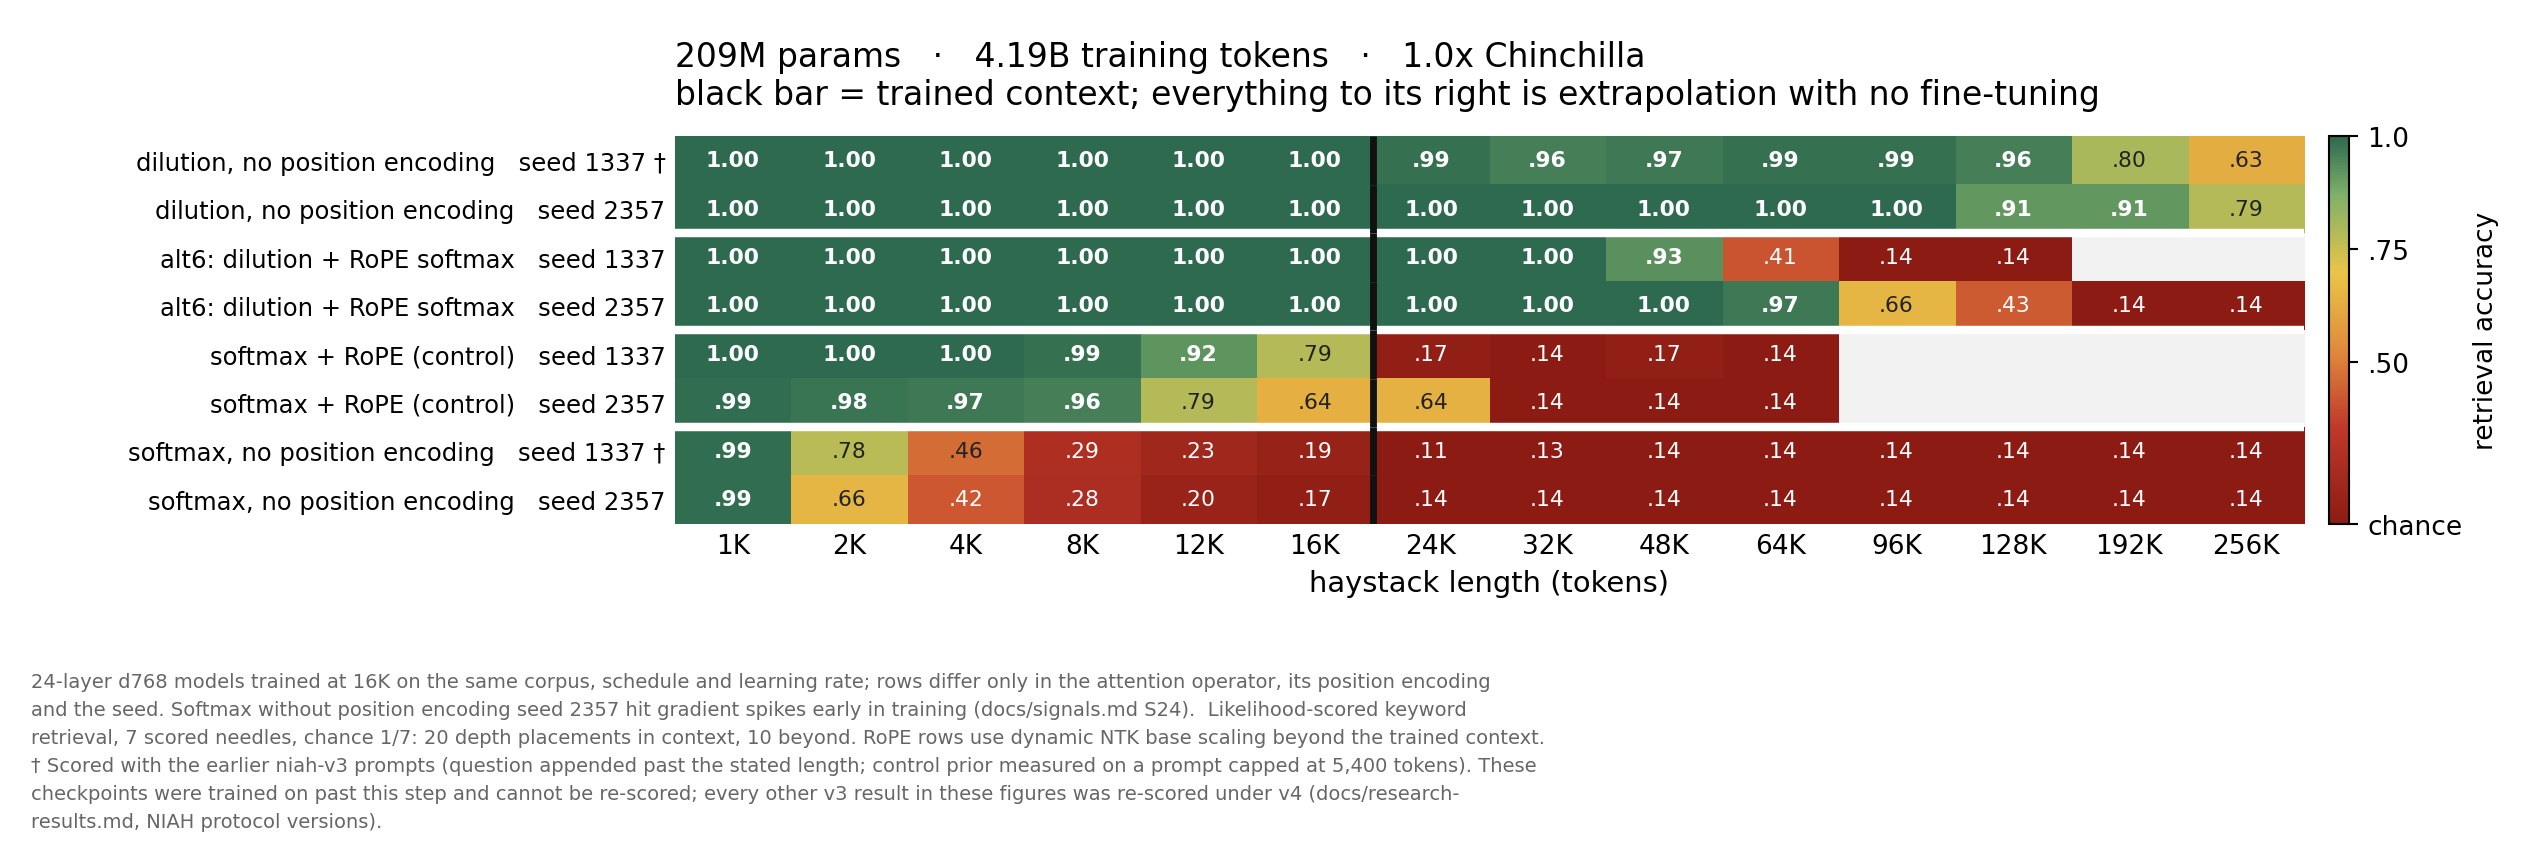
\includegraphics[width=\linewidth]{retrieval-209m-1x.png}
\caption{NIAH retrieval past the training context, 209M parameters, 16K training context, 1$\times$
Chinchilla, every seed. Cells right of the black bar are extrapolation with no fine-tuning. Rows
marked $\dagger$ were scored with an earlier protocol version whose checkpoints no longer exist at
this step; all other results were re-scored with the current one.}
\label{fig:retrieval}
\end{figure}

\begin{table}[t]
\centering\small
\begin{tabular}{@{}lcccc@{}}
\toprule
arm (209M, 16K, 1$\times$) & val.\ loss (two seeds) & NIAH at 16K & retrieval beyond 16K & tok/s \\
\midrule
alt6 (RoPE softmax + dilution) & \textbf{3.0385 / 3.0399} & 1.00 / 1.00 & 3--4$\times$ with NTK & 44.0K \\
dilution, no position encoding & 3.0569 / 3.0548 & 1.00 / 1.00 & \textbf{8$\times$ in both seeds} & 33.4K \\
softmax + RoPE & 3.0883 / 3.0787 & 0.79 / 0.64 & 1.5$\times$ in one seed & \textbf{71.9K} \\
softmax, no position encoding & 3.2118 / 3.2907$^*$ & 0.19 / 0.17 & chance & 74.7K \\
\bottomrule
\end{tabular}
\caption{The 209M comparison. $^*$This seed hit a burst of gradient spikes and never recovered the
loss. NIAH chance is 0.14.}
\label{tab:main}
\end{table}

\subsection{Length extrapolation comes from the operator}

With no position encoding on either side, dilution retrieves 1.00 across its 16K context and
0.91--1.00 out to 128K in both seeds, then degrades gradually (0.80--0.91 at 12$\times$, 0.63--0.79 at
16$\times$); softmax reaches 0.17--0.19 at its own trained context and chance past it
(Figure~\ref{fig:retrieval}, Table~\ref{tab:main}; \ledger{S17, S24}). Dilution without position
encoding also beats softmax \emph{with} RoPE on loss. No tested softmax configuration sustains strong
retrieval far beyond its training context: the 16K-trained controls are at chance by 2$\times$ (one
softmax + RoPE seed holds 0.64 at 1.5$\times$ with NTK scaling), and the 1K-trained controls keep
partial retrieval near 2$\times$ (0.56 / 0.39 without position encoding) before degrading. The
RoPE-bearing dilution and hybrid configurations also degrade eventually; NTK scaling extends some of
them but does not remove the degradation.

\subsection{Long-document perplexity}\label{sec:pg19}
\begin{figure}[t]
\centering
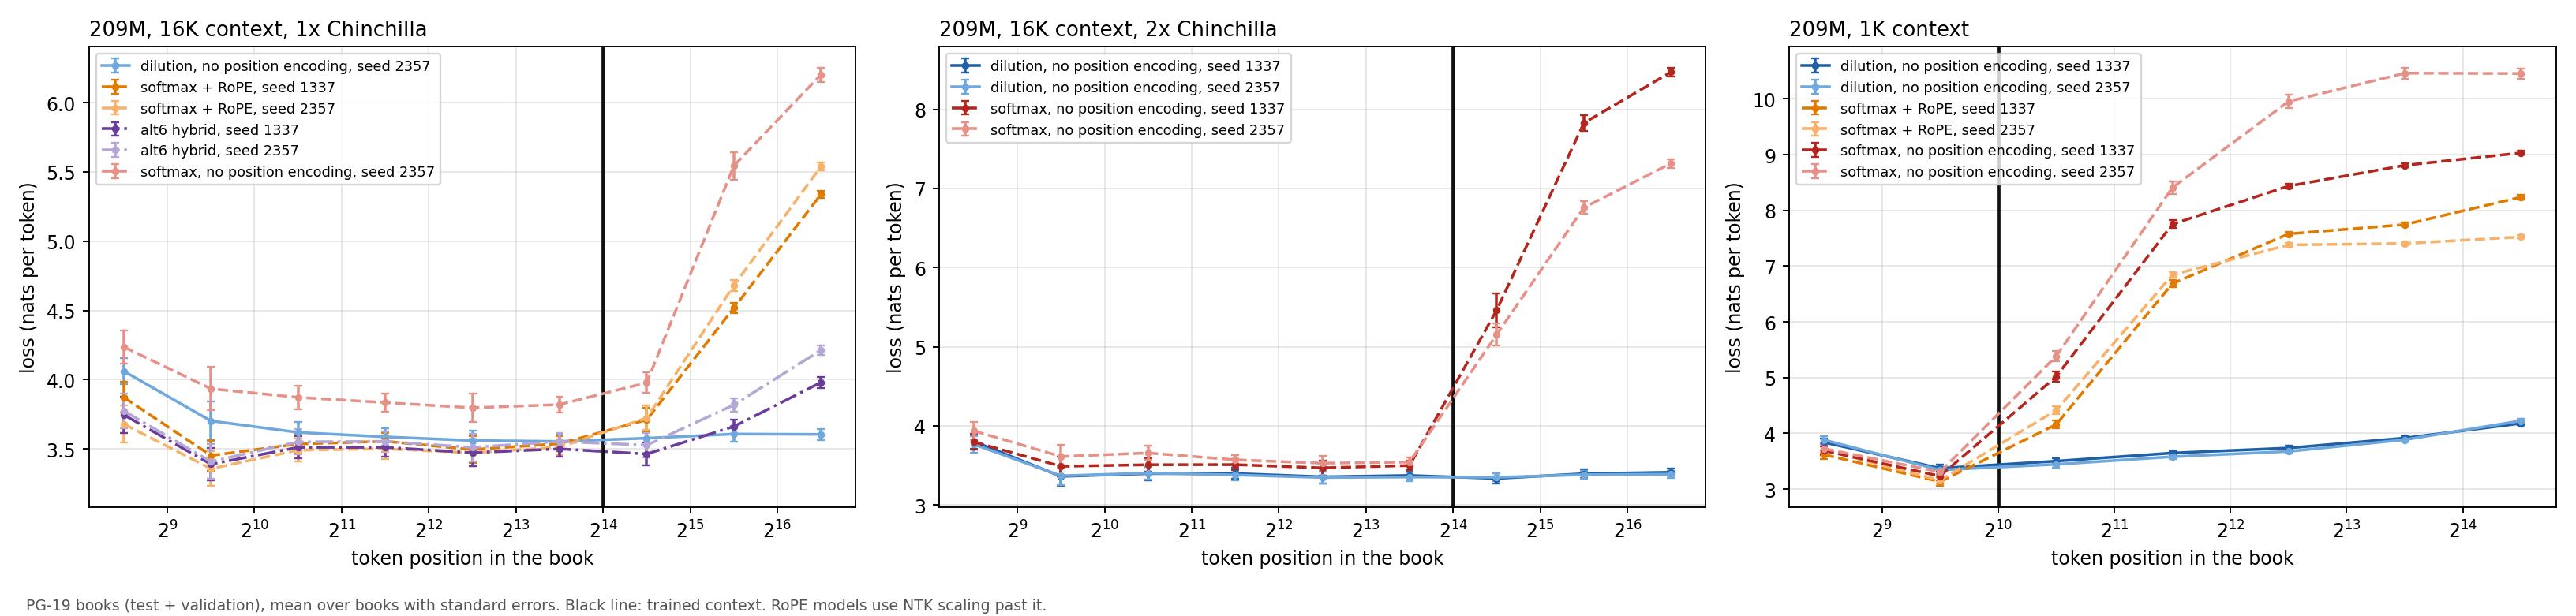
\includegraphics[width=\linewidth]{pg19-perplexity-209m.png}
\caption{Loss by position on PG-19 books (29 books of at least 128K tokens for the 16K models, 120 of
at least 32K for the 1K models), mean over books with standard errors. Black line: trained context.
RoPE models use NTK scaling past it.}
\label{fig:pg19}
\end{figure}

Retrieval is a synthetic test; loss by position on long real documents is the standard measurement
of length extrapolation. Each model reads the first 128K (16K models) or 32K tokens (1K models) of long
PG-19 books~\cite{pg19} teacher-forced, and the loss at every position is averaged within doubling
position ranges (Figure~\ref{fig:pg19}; \ledger{S27}). Past the trained context the 16K dilution models
stay flat to 8$\times$, within 0.05 nats of their in-context loss. Paired over books, softmax + RoPE with
NTK scaling is 0.9--1.1 nats worse than dilution at 4$\times$ and 1.7--1.9 at 8$\times$ (at 2$\times$ the
difference, 0.13--0.15, is within noise), and softmax without position encoding is 2.6--5.1 nats
worse at 8$\times$. alt6 matches dilution at 2$\times$ and degrades from 4$\times$. The 1K dilution models degrade
gradually (+0.1 nats at 2$\times$, +0.85 at 32$\times$), while every 1K softmax model rises by 1.0--2.1 nats
at 2$\times$ and 3.5--5.1 by 4$\times$.

Inside the trained context the comparison differs from the in-domain validation slice. On these books,
which are far from the training data, dilution trails softmax + RoPE by 0.05--0.08 nats at 16K and by
0.18--0.24 at 1K, and trails softmax without position encoding by 0.09--0.15 at 1K, most at the start of
each book; on FineWeb-Edu validation text the same checkpoints put dilution 0.02--0.03 ahead of softmax +
RoPE at 16K and 0.036 behind it at 1K. We have not tested why.

\subsection{Extrapolation range varies by seed}

Dilution's loss replicates closely (seeds agree to within about 0.007 nats in every cell measured,
0.002--0.004 at 209M), but its reach does not.
Trained on to 2$\times$ Chinchilla, both dilution seeds reach 2.857 / 2.854 and keep in-context
retrieval, but one then holds only to about 2$\times$ (0.54 at 64K) while the other stays near-flat
(0.97 at 64K, 0.83 at 128K). At 1K context the two seeds reach 4$\times$ and 8$\times$. At 64M without
position encoding, in-context retrieval itself forms in only about two seeds of three, at identical
loss; the failed seeds never grow the strong retrieval head (53--76\% of one head's attention on the
answer token in layers 6--9) that healthy seeds have. RoPE on alternate layers makes retrieval form in
all three seeds (\ledger{S22--S24}). Extrapolation should be reported as a range over seeds.

\subsection{Loss depends on context length}

Once each operator has its best position mode, softmax + RoPE is ahead by 0.036 nats at 1K (209M,
two seeds), the two are level within 0.007 at 8K (64M), and dilution leads at 16K: by 0.028 without
position encoding and 0.044 for alt6 at 209M, and by 0.077--0.092 at 64M over three seeds. Earlier
comparisons against learned-position softmax reported 0.19--0.43 nats and mostly measured that
baseline's failure (\ledger{S1, S5--S9, S11, S21--S24}). These margins are on in-domain
validation text; on out-of-domain books (Section~\ref{sec:pg19}) dilution trails inside the trained
context.

\subsection{Generated text}

\begin{table}[t]
\centering\small
\begin{tabular}{@{}lccc@{}}
\toprule
209M models (nucleus sampling) & inside the trained context & 2$\times$ past it & 4$\times$ past it \\
\midrule
16K, 1$\times$: dilution, no position encoding & 1.09--1.13 & \textbf{1.14} & \\
\quad softmax + RoPE & 1.09--1.15 & 1.87 / 2.15 & \\
\quad alt6 & 1.06--1.10 & 1.20 / 1.20 & \\
16K, 2$\times$: dilution, no position encoding & 1.00--1.04 & \textbf{1.00 / 1.02} & \\
\quad softmax, no position encoding & 1.05--1.14 & 3.33 / 2.31 & \\
1K: dilution, no position encoding & 1.07--1.10 & \textbf{1.12 / 1.11} & \textbf{1.16 / 1.13} \\
\quad softmax + RoPE & 1.05--1.09 & 2.45 / 2.58 & 2.97 / 2.62 \\
\quad softmax, no position encoding & 1.07--1.10 & 2.26 / 2.37 & 2.25 / 2.77 \\
human continuation & 0.65--0.70 & & \\
\bottomrule
\end{tabular}
\caption{Judge bits per byte of 256-token continuations (lower is more natural; pairs are two seeds).
128--256 prompts per cell.}
\label{tab:gen}
\end{table}

Inside the trained context, judged sample quality tracks loss (Table~\ref{tab:gen}; \ledger{S25}):
dilution is level with softmax + RoPE at 16K, 0.03--0.12 bits per byte better than softmax without
position encoding at 2$\times$ Chinchilla, and about 0.01 behind softmax + RoPE at 1K, where softmax has
the better loss. The test resolves loss gaps of about 0.2 nats (training the same dilution seed from
1$\times$ to 2$\times$ improves its samples by 0.05--0.11), not a few hundredths. Past the trained context,
all the softmax models tested write incoherent text at 2--4$\times$, and scored teacher-forced they
assign the human continuation 6--9 nats per token; dilution's samples stay within 0.06 of their
in-context quality and its loss on the human text within 0.04. Because the judge sees only the last
4,096 tokens, this shows that dilution remains a working language model past its trained window, not
that it uses information from far back. Greedy decoding loops in every model at this scale.

\subsection{Attention structure}

In three sampled layers of one 1,024-token window per model, averaged over heads, dilution strongly
suppresses the token-0 sink: no sampled dilution layer puts more than 0.028 of its attention there,
against 0.14--0.75 for 209M softmax without position encoding and 0.25--0.32 with RoPE. At depth its
load is less concentrated across keys at similar per-query selectivity. Neither statistic tracks
extrapolation range: two dilution seeds that differ in reach have the same sink and key concentration
(\ledger{S20}). These are snapshots of trained models, not a causal account.

\section{Related work}

\emph{Temporal attention and coverage.} Temporal attention~\cite{sankaran,paulus} is the closest
equation-level precedent (Section~2); coverage models~\cite{tu,mi,see} feed accumulated attention back
into a learned score or loss rather than dividing by it, and See et al.\ found post-hoc temporal
division harmful in their summariser. \emph{Balanced and competitive attention.}
Sinkformers~\cite{sinkformers} balance rows and columns iteratively; Flowformer~\cite{flowformer} and
Slot Attention~\cite{slot} create competition through conservation or normalisation over slots; none
divides a causal softmax bid by prior demand. \emph{Sinks and caches.} StreamingLLM and
StableMask~\cite{streamingllm,stablemask} characterise and manage the attention sink; H2O~\cite{h2o}
uses accumulated attention to evict cache entries. \emph{Position encoding and length
generalisation.} RoPE~\cite{rope}, NoPE~\cite{nope}, position interpolation~\cite{pi} and
YaRN/NTK scaling~\cite{yarn} target extrapolation through the position signal; our result is an
operator-level effect measured with position encoding held fixed. \emph{Kernels.}
FlashAttention~\cite{flashattention} and FlexAttention~\cite{flexattention} fuse row-local softmax
attention; dilution's column prefix sum needs a different decomposition.

\section{Limitations}

\begin{itemize}
\item Scale: 64M and 209M parameters, one tokenizer and one corpus family. Whether the effects hold at
billions of parameters is untested.
\item Retrieval is measured with a synthetic, likelihood-scored keyword test. Generation is tested for
local fluency only. Long-range use of information in free generation, retrieval by generation and
long-context reasoning benchmarks are untested.
\item Seeds: two per arm at 209M, three at 64M. Extrapolation range is seed-dependent.
\item Cost: dilution trains 1.3$\times$ (1K) to 2.2$\times$ (16K) slower than SDPA softmax; the heaviest
backward pass is latency-bound and further gains need a lower-level implementation.
\item In-context loss out of domain: on long PG-19 books dilution trails softmax + RoPE inside the
trained context by 0.05--0.08 nats at 16K and 0.18--0.24 at 1K, although it is level or ahead on
in-domain text.
\item Mechanism: why dilution extrapolates is not established causally.
\end{itemize}

\section{Reproducibility}

The release contains the operator's fp32 reference and fused kernels with parity tests; training and
evaluation code; the configuration, metrics and data provenance of the 101 runs behind the published
results (the wider study, including short screens and exploratory runs outside this report's scope,
comprised about 200); every result file behind the tables and figures, including per-sample sampling
metrics from which a script recomputes every published statistic; the final weights of the 16 209M
models on Hugging Face (\url{https://huggingface.co/Royer-Research-Labs}); and an evidence ledger that records
each finding with its runs, including corrections and withdrawn claims. Every number in this
report traces to a run record and a result file in the repository. The software release is archived on Zenodo (\href{https://doi.org/10.5281/zenodo.23073037}{doi:10.5281/zenodo.23073037}).

\begin{thebibliography}{99}\small
\bibitem{sankaran} B.~Sankaran, H.~Mi, Y.~Al-Onaizan, A.~Ittycheriah. Temporal attention model for neural machine translation. arXiv:1608.02927, 2016.
\bibitem{paulus} R.~Paulus, C.~Xiong, R.~Socher. A deep reinforced model for abstractive summarization. ICLR 2018.
\bibitem{see} A.~See, P.~J.~Liu, C.~D.~Manning. Get to the point: summarization with pointer-generator networks. ACL 2017.
\bibitem{tu} Z.~Tu, Z.~Lu, Y.~Liu, X.~Liu, H.~Li. Modeling coverage for neural machine translation. ACL 2016.
\bibitem{mi} H.~Mi, B.~Sankaran, Z.~Wang, A.~Ittycheriah. Coverage embedding models for neural machine translation. EMNLP 2016.
\bibitem{sinkformers} M.~E.~Sander, P.~Ablin, M.~Blondel, G.~Peyr\'e. Sinkformers: Transformers with doubly stochastic attention. AISTATS 2022.
\bibitem{flowformer} H.~Wu, J.~Wu, J.~Xu, J.~Wang, M.~Long. Flowformer: linearizing Transformers with conservation flows. ICML 2022.
\bibitem{slot} F.~Locatello et al. Object-centric learning with slot attention. NeurIPS 2020.
\bibitem{streamingllm} G.~Xiao, Y.~Tian, B.~Chen, S.~Han, M.~Lewis. Efficient streaming language models with attention sinks. ICLR 2024.
\bibitem{stablemask} Q.~Yin et al. StableMask: refining causal masking in decoder-only Transformer. ICML 2024.
\bibitem{h2o} Z.~Zhang et al. H$_2$O: heavy-hitter oracle for efficient generative inference of large language models. NeurIPS 2023.
\bibitem{rope} J.~Su, Y.~Lu, S.~Pan, A.~Murtadha, B.~Wen, Y.~Liu. RoFormer: enhanced Transformer with rotary position embedding. arXiv:2104.09864, 2021.
\bibitem{nope} A.~Kazemnejad, I.~Padhi, K.~Natesan Ramamurthy, P.~Das, S.~Reddy. The impact of positional encoding on length generalization in Transformers. NeurIPS 2023.
\bibitem{pi} S.~Chen, S.~Wong, L.~Chen, Y.~Tian. Extending context window of large language models via positional interpolation. arXiv:2306.15595, 2023.
\bibitem{yarn} B.~Peng, J.~Quesnelle, H.~Fan, E.~Shippole. YaRN: efficient context window extension of large language models. ICLR 2024.
\bibitem{flashattention} T.~Dao, D.~Y.~Fu, S.~Ermon, A.~Rudra, C.~R\'e. FlashAttention: fast and memory-efficient exact attention with IO-awareness. NeurIPS 2022.
\bibitem{flexattention} J.~Dong, B.~Feng, D.~Guessous, Y.~Liang, H.~He. FlexAttention: a programming model for generating fused attention variants. MLSys 2025.
\bibitem{chinchilla} J.~Hoffmann et al. Training compute-optimal large language models. NeurIPS 2022.
\bibitem{fineweb} G.~Penedo et al. The FineWeb datasets: decanting the web for the finest text data at scale. NeurIPS 2024 Datasets and Benchmarks.
\bibitem{pg19} J.~W.~Rae et al. Compressive Transformers for long-range sequence modelling. ICLR 2020.
\bibitem{smollm2} L.~B.~Allal et al. SmolLM2: when smol goes big, data-centric training of a small language model. arXiv:2502.02737, 2025.
\bibitem{unlikelihood} S.~Welleck, I.~Kulikov, S.~Roller, E.~Dinan, K.~Cho, J.~Weston. Neural text generation with unlikelihood training. ICLR 2020.
\bibitem{nucleus} A.~Holtzman, J.~Buys, L.~Du, M.~Forbes, Y.~Choi. The curious case of neural text degeneration. ICLR 2020.
\end{thebibliography}

\end{document}
